\thispagestyle{empty}
\chapter{Molecular evolution}
{
	\hypersetup{linkcolor=GREYDARK}
	\minitoc
}

\label{sec:intro}

From the discovery of evolution to today knowledge, the understanding of the mechanisms from which the diversity of life and complexity emerges has seen dramatic changes, and revolution.
One such revolution is called molecular evolution, a recent scientific fields, emerging at the crossroad of evolutionary biology which had seen tremendous theoretical development in the nineteenth and twentieth century, and molecular biology which recruited advances in chemistry and had seen many technical revolutions.
Being both empirical and theoretical biology, molecular evolution borrows strength from the amount of empirical data available in molecular biology, and the predictive power of evolutionary biology.
From the difference of molecular sequences observable between individuals of the same population, or difference of sequences between species, we can wonder what are the processes generating such diversity?
What are the forces governing such evolutionary mechanisms?
Can we quantify the relative strength of these forces, shaping both nowadays populations but also ancient and sometimes extinct lineages?
In a nutshell, molecular evolution leverages the patterns of sequences distribution carried by individuals in order to uncover evolutionary mechanisms shaping organisms evolution and their ancestral lineages, while at the same time shining light on cellular and molecular processes allowing organism to live and reproduce.

\section{Historical perspective}

This section will recall theoretical frameworks, assumptions and limitations on which molecular evolution is based.
It will emphasis the milestones and their respective contribution, while doing its best to highlight the undertaken paths which have been forgotten with time.
It is a modest attempt neither exhaustive nor accurate, imprinted with ideology of our current society on how we perceive and interpret past discoveries. 
Moreover, this introduction will highlight a few names, while the bulk of the rigorous assessment and develpoment of molecular evolution has been done by unmentioned and sometimes forgotten scientists.

\subsection{Population-genetic}
Molecular evolution is theoretically build upon the framework of population-genetic, which in turn historically emerged as an unifying theory between Mendelian inheritance and quantitative genetic, in the early twentieth century.
Originally, Johann Gregor Mendel (1822-1884) established the statistical laws governing heredity of discrete characters through  hybridisation experiments on the garden pea plant \textit{Pisum sativum} between 1857 and 1864.
This model of inheritance was rediscovered and confirmed in the early twentieth century independently by botanists Hugo de Vries (1848-1935), Carl Correns (1864-1933) and Erich von Tschermak (1871-1962) \citep{dunn2003gregor}.

Models of Mendelian inheritance where deemed incompatible by biometricians, while the crux of the argument revolved around the evolution of continuous characters\footnote{Incompatibility between continuous and discrete evolution can actually be traced back to debates between Jean-Baptiste de Lamarck (1744-1829) defending gradual changes and Georges Cuvier (1869-1932) supporting punctual catastrophic changes, in the late eighteenth century.}.
Broadly speaking, supports of Mendelian genetic believed that evolution was driven by mutations transmitted by the discrete segregation of alleles, which biometricians rejected on the basis that it would necessarily imply discontinuous evolutionary leaps \citep{bowler2003evolution}.
On the other hand, biometricians claimed that variation was continuous, which mendelian geneticist rejected on the basis variations measured by biometricians were too small to be subject to selection \citep{provine2001origins}.

Statistician Ronald A.\ Fisher reconciled both theories, first by proving mathematically that mutiple discrete loci could result in a continuous variation \citep{fisher1919xv}.
Secondly, \citet{fisher1930genetical, haldane1932causes} proved that natural selection could change \gls{allele} frequencies in a population. 
Fisher and Haldane hence articulated selection on continuous traits with discrete underlying genetic inheritance, completed by the work of \citet{wright1932roles} on combinations of interacting genes.
Altogether, they laid the foundations of population genetics, a discipline which basically integrated Mendelism, Darwinism and biometry, easing the debate between continous and gradual evolution\footnote{This debate was revived by paleontologists \citet*{Gould1972}. As of today it is admitted that both macroevolutive patterns of ponctual and gradual changes can be found.}.

The emergence of this new field of study was the first step towards the development of a unified theory of evolution named the ‘modern synthesis’ \citep{huxley1942evolution}, defined on the basis that natural selection acts on the heritable variation supplied by mutations \citep{mayr1959where,stebbins1966processes,dobzhansky1974chance}.

\subsection{Central dogma of molecular biology}
During the theoretical development of population-genetic, the support of heredity was largely unknown, the terminology of gene, alleles and loci where theoretical and not grounded on chemical first principles.
The first evidence that deoxyribonucleic acid (\acrshort{DNA}) carries genetic information is in the work of \citet{Avery1944}, after bacteria treated with a deoxyribonuclease enzyme failed to transform, while otherwise transforming, even when treated by protease.
The chemical composition of \acrshort{DNA} was later refined by \citet{Chargaff1950}, whom found that the amounts of adenine (A) and thymine (T) in \acrshort{DNA} were roughly the same as the amounts of cytosine (C) and guanine (G).
Most importantly, the relative amounts of guanine, cytosine, adenine and thymine bases were found to vary from one species to another, which provided evidence that \acrshort{DNA} could encodes genetic information, through a four letter molecular alphabet.

Ultimately, the double-helix structure of \acrshort{DNA} was deciphered by \citet{franklin1953molecular,watson1953molecular,wilkins1953molecular}.
More precisely, \acrshort{DNA} consists of two interwoven strands of nucleotides, each of which contains an identical phosphate group, an identical $5$-carbon sugar (deoxyribose) and a variable base which define the four nucleotide: T, C, A and G.
Apart from being different molecules, bases are also hybridizing via hydrogen bonds, which are weak attractive forces between hydrogen and either nitrogen or oxygen.
This hybridization explains that the two strands of \acrshort{DNA} are interwoven due to base pair complementarity, where a specific base on one strand is aligned with its complement on the other strand.
More precisely, the complementary bases are:
\begin{itemize}
	\item A with T, through two hydrogen bonds.
	\item G with C, through three hydrogen bonds which are stronger than A-T bonds. 
\end{itemize}
It is important to note the two strands are oriented, a constrained imposed by the asymmetry of the deoxyribose, where one end is called the ${\it 5}'$ end and the other ${\it 3}'$ end\footnote{The naming come from the numbering of carbon atoms of the asymmetric sugar molecule ($5$ of them) on which the end is attached.}. 
This means that two strands will only hybridize if they are reverse complement, such that that the sequence of one strand when read from $5'$ to $3'$ is complementary to the sequence of the other strand read from $3'$ to $5'$.

Ultimately, the information contained by each strand of \acrshort{DNA} is redundant, and this redundancy is leveraged during replication of the \acrshort{DNA}.
During the cell cycle, the \acrshort{DNA} double strand is split into its two separate strands, each of them used as a template to synthesize its complementary strand, resulting in two copies of the original double-stranded \acrshort{DNA}.

Once understood that molecular structure of \acrshort{DNA} and its role has a support of heredity, the guest to understand the transfer of information between \acrshort{DNA} and protein \cite{Crick1958} resulted in the determination of the genetic code, the translation table from triplet of nucleotides (\gls{codon}) to amino-acids, and of the central dogma of molecular biology detailing the process of protein synthesis \cite{Crick1970}.
Proteins are synthesized in a two-step process called gene expression.
First, an messenger ribonucleic acid (mRNA) transcript is synthesized from \acrshort{DNA}, containing the same information since \acrshort{RNA} is also formed by 4 bases, where Thymin (T) is replaced by uracil (U), though the three other bases are the same. 
Second, mRNA is matured and spliced to form a mature \acrshort{RNA}, which is read and interpreted by ribosomes to synthesize a protein in a process called translation. 
More broadly, the central dogma of molecular biology states that the determination of sequence from nucleic acid to nucleic acid, or from nucleic acid to protein may be possible, but transfer from protein to protein, or from protein to nucleic acid is impossible.
It is worth noting that each protein is encoded by its \acrshort{DNA} sequence, although the same \acrshort{DNA} sequence can produce many different proteins through a process called alternative splicing.

As the support of heredity, \acrshort{DNA} gained a central role in evolutionary biology, and development of polymerase chain reaction (PCR), Sanger sequencing and their subsequent refinement revolutionized the availability of empirical data on which to test the theoretical prediction and development of population genetics.

\subsection{Neutral theory}

Although an unifying theory, population-genetics remained rather theoretical for some time because it deals with the concept of gene frequencies and has no direct way to connect unambiguously to conventional dataset obtained at the phenotypic level.
With the advent of molecular genetics, it became possible to study the variability of nucleic and protein sequences within a species, as well as in related organism such as to estimate the rate at which allelic genes are substituted.

From protein sequences in related species, it was then observed that a given protein rate of substitution is about the same in many diverse lineages, where the substitutions seemed to be random rather than having a specific pattern.
Additionally, from DNA sequences in related species, it was observed that the overall rate of DNA substitutions is very high, of least one nucleotide base per genome every two years in a mammalian lineage.
On the other hand, from the variability of protein sequences in the same population, electrophoretic methods suddenly unveiled a wealth of genetic variability, such that the proteins produced by a large fraction of the genes in diverse organisms were found to be polymorphic, and in many cases the protein polymorphism had no visible phenotypic effects and no obvious correlation.
Altogether, these observation lead Motoo Kimura to propose the \gls{neutral} theory of molecular evolution \citep{kimura1968evolutionary,kimura1991neutral,kimura1986dna}.
Neutral theory claimed that most mutations are adaptively \gls{neutral} and thus become fixed in populations through the cumulative effect of \gls{drift}.
Tomoko Ohta later incorporated weakly selected mutation into the \gls{nearly-neutral} theory \citep{ohta1973slightly}, such that selection effect in the order of inverse population size are negligible and behaves neutrally.
Altogther, that many protein polymorphisms must be selectively neutral or nearly so and must be maintained in a population by the balance between mutational input and random extinction, and as a consequence, the majority of the nucleotide substitutions in the course of evolution must be the result of the random fixation of neutral or nearly-neutral mutants rather than the result of positive Darwinian selection.

Selectionists maintain that for a mutant allele to spread through a species it must have some selective advantage, although they admit that an allele that is itself neutral may occasionally be carried along by "hitchhiking" on a gene that is selected for and with which it is closely linked, and may thus reach a high frequency.
Neutralists, on the other hand, contend that some mutants can spread through a population on their own without having any selective advantage. If a mutant is selectively equivalent to preexisting alleles, its fate is left to chance.
Its frequency fluctuates, increasing or decreasing fortuitously over time, because only a relatively small number of gametes are "sampled," out of the vast number of male and female gametes produced in each generation, and are therefore represented in individuals of the next generation.
As of today, it is widely accepted that both \gls{drift} and natural selection participate in the evolution of genomes: the controversy is no longer strictly dichotomous but rather concerns the quantitative contributions of adaptive and of non-adaptive evolutionary processes, and their articulation.

\section{Population-genetics of sequences}
In molecular evolution, available sequences are leveraged to reconstruct ancestral lineages and unveils evolutionary mechanisms generating this diversity of sequences, or in other words, we are reconstructing ancestral path undertaken by organisms using available knowledge today.
But ultimately, such effort to infer mechanisms backward in time requires a theoretical model that generate diversity forward in time, where we can play this model forward and derive how likely such model would generate the pattern of sequence distribution we observe.
One such predictive theoretical framework is population-genetic, entailed with its assumptions and limitations.
This section thus recall the Wright-Fisher model of sequence evolution and its assumptions, such as to relate parameters of evolution such as mutation, selection and drift to observable patterns in molecular sequences such as the probability of fixation of a mutant \gls{allele}, as well as the expected number of copies of the derived \gls{allele} we should observe.
These relationships between underlying evolutionary forces and patterns of sequence evolution will subsequently be leveraged and recruited in the next section to derive models of sequence substitutions parameterized by mutation, selection and drift.
Although the mathematical proof for such results are out of the scope of this manuscript, model definitions and assumptions are stated. 
Such effort is meant to clearly define the models and its parametrization from the ground up. 

\subsection{Wright-Fisher process}

The Wright-Fisher model describe the change in frequency of a \gls{polymorphic} gene with two alleles in a \gls{diploid} population over time. 
The frequency of the mutant \gls{allele} $A$ is denoted $p$ while the frequency of the resident $B$ alleles is $1-p$.
Selection is assumed to occurs between the zygotic and the adult stage, called post-zygotic selection, where the \gls{allele} $A$ has an additive selection coefficient (no dominance) denoted $s$.
More precisely, the ability to survive and produce offspring that eventually become reproductive, a measure called absolute Wrightian fitnesses of the $3$ different possible genotypes are shown in table \ref{table:fitnesses} as a function of the selection coefficient.

\begin{table}[H]
	\centering
	\begin{tabular}{|l|ccc|}
		\hline
		\textbf{Genotype} & $\bm{AA}$ & $\bm{AB}$ & $\bm{BB}$ \\
		\hline\hline
		Absolute Wrightian fitness ($W$) & $1+2s$ & $1+s$ & $1$ \\
		\hline Hardy-Weinberg frequency & $p^2$ & $2p(1-p)$ & $(1-p)^2$ \\
		\hline Relative Wrightian fitness & $\dfrac{1+2s}{1+2ps}$ & $\dfrac{1+s}{1+2ps}$ & $\dfrac{1}{1+2ps}$ \\
		\hline
	\end{tabular}
	\caption[Fitnesses of the different genotypes]{Fitnesses of the different genotypes}\label{table:fitnesses}
\end{table}

Under the Hardy-Weinberg equilibrium of the population, the mean fitness in the population is a function of the selection coefficient and frequency of alleles as:
\begin{align}
\bar{W} &= (1+2s)p^2 + (1+s)2pq + q^2 \\
&= 1 + 2ps,
\end{align}
And the relative fitness\footnote{Analogous explanation between absolute and relative fitness can be found in economics, where absolute fitness correspond to wealth generation, while relative fitness is just transfer of wealth from one to another \citep{Masel2016}.} of the three different genotypes are also shown in table \ref{table:fitnesses}. 

Adults contribute to the next generation proportionally to the fitness of their genotype, and assuming a discrete generation and random mating between individuals, the genotype frequencies in the zygotes match the Hardy-Weinberg distribution if no recurrent mutation is allowed.
Altogether, the frequency $p'$ of gametes bearing the $A$ \gls{allele} produced by the adults passed down to the next generation is:
\begin{align}
p' & = p^2 \dfrac{1+2s}{1+2ps} + p(1-p)\dfrac{1+s}{1+2ps}\\
& = p\dfrac{1+s(1+p)}{1 + 2ps}
\end{align}

\begin{figure}[H]
	\begin{center}
		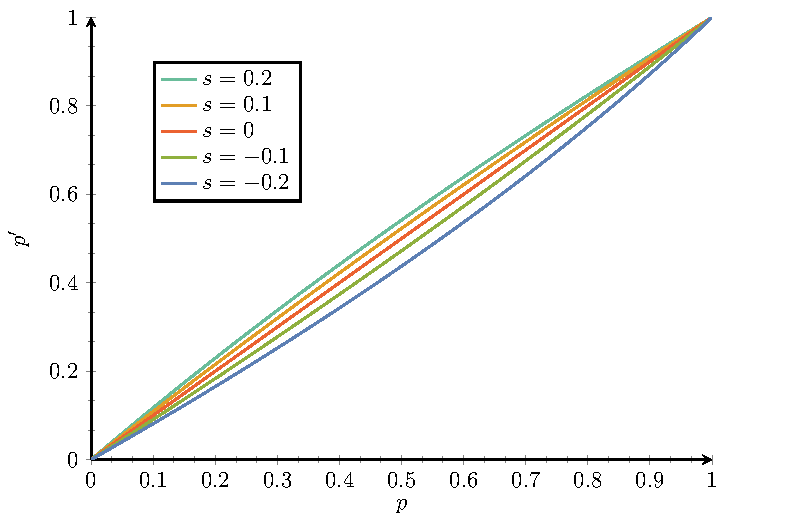
\includegraphics[width=0.8\textwidth, page=1] {figures.pdf}
	\end{center}
	\caption[Frequency of derived \gls{allele} after a generation]{Frequency of derived \gls{allele} after a generation. Positive selection coefficient ($s > 0$) result in increased derived \gls{allele} frequency at the next generation, which is intuitively expected. The effect is stronger when the derived \gls{allele} frequency is close to $0.5$, intuitively because the poll of both alleles must be sufficiently large such that they can be replaced. It is worth noting that even for strong selection coefficient ($s=0.2$), completely unrealistic in real population, the difference in frequency from one generation to the next is subtle.}
\end{figure}

The population is considered discrete and consists of a fixed number of \gls{diploid} individuals $\Ne \gg 1$, where the number of copies of the derived \gls{allele} $A$ present at the current generation is denoted $i$ and $p=i / 2\Ne $ 
The probability $\mathcal{P}_{ij}$, that there are $j$ copies of the derived \gls{allele} $A$ present at the next generation is given by the binomial distribution:
\begin{align}
\mathcal{P}_{ij} & = \binom{2 \Ne}{j} \left( p' \right)^j \left(1 - p' \right)^{2 \Ne -j} \\
				 & = \binom{2 \Ne}{j} \left( p\dfrac{1+s(1+p)}{1 + 2ps} \right)^j \left(1 - p\dfrac{1+s(1+p)}{1 + 2ps} \right)^{2 \Ne -j}
\end{align}

These {transition} probabilities define a discrete-space and discrete-time Markov process.
However, it has been shown to be extremely difficult to explicitly derive formulas for several quantities of evolutionary interest.
However, as the size of the population approaches infinity (i.e. $ \Ne \to \infty$), and assuming that the scaled selection pressure ($\Ne s $) remain constant, the discrete Markov process given above can be closely approximated by continuous-time and continuous-space diffusion process.\\

\subsection{Probability of fixation}
Starting from an initial frequency, the process eventually reach absorption, whether the derived \gls{allele} invade the population or dies out. 
Under the continuous-time and continuous-space diffusion process approximation, partial differential equations know as Kolmogorov backward equation allow to derive the probability of such events. 
If the selection coefficient is weak ($|s| \ll 1$), the probability of fixation ($P_{\mathrm{fix}}$) of a derived \gls{allele} with selection coefficient $s$ and initial frequency $p$ was derived by \citet{Kimura1962}:
\begin{align}
P_{\mathrm{fix}}(s, \Ne, p) & = \dfrac{1 - \e^{-4 \Ne p s }}{1 - \e^{-4 \Ne s}},\\
			     & = \dfrac{1 - \e^{- p S }}{1 - \e^{-S}},
\end{align}
where $S = 4 \Ne s$ is the scaled selection coefficient.
\begin{figure}[H]
	\begin{center}
		\includegraphics[width=0.8\textwidth, page=3] {figures.pdf}
	\end{center}
	\caption[Probability of fixation]{Probability of fixation. The selection coefficient of the derived \gls{allele} is scaled by population size $S=4 \Ne s$. In contrast to changes of frequency during a generation, the probability of fixation is sensitive to very weak selection coefficient ($|s| \ll 1$), as long as the scaled selection coefficient is not negligible ($|S| > 1$). Intuitively, selective effects are magnified by population size because the fixation is the inherently the resultant of the trajectory overall, integrating small effects throughout the lifespan of the \gls{allele}. }
\end{figure}

An interesting special case is obtained for a new mutation appearing in the population.
Because it is a single mutant the derived \gls{allele} initial frequency is $p = 1 / 2 \Ne$, and the probability of fixation ($P_{\mathrm{fix}}$) if given by:
\begin{align}
	P_{\mathrm{fix}}(s, \Ne) & = \dfrac{1 - \e^{-2 s}}{1 - \e^{-4 \Ne s}} \\
	 & \simeq  \dfrac{2 s }{1 - \e^{-4 \Ne s}}
\end{align}
The special case of a \gls{neutral} \gls{allele} can be obtained by taking the limit when $s$ goes to $0$.
\begin{align}
P_{\mathrm{fix}}(0, \Ne) & = \dfrac{1}{2 \Ne}
\end{align}
Altogether, the fixation probability of a selected \gls{allele} relative to a \gls{neutral} \gls{allele} is solely dependent on the scaled selection coefficient:
\begin{align}
\dfrac{P_{\mathrm{fix}}(s, \Ne)}{P_{\mathrm{fix}}(0, \Ne)} & \simeq 2 \Ne \dfrac{2s}{1 - \e^{-S}} \\
& \simeq  \dfrac{S}{1 - \e^{-S}}
\end{align}
\begin{figure}[H]
	\begin{center}
		\includegraphics[width=0.8\textwidth, page=2] {figures.pdf}
	\end{center}
	\caption[Relative fixation probability]{Fixation probability of a selected \gls{allele} relative to a \gls{neutral} \gls{allele}.
	For a substantive negative scaled selection coefficient ($s \leq -1/\Ne$, red filled area), the probability of fixation is greatly reduced (by an exponential factor), and \gls{allele} can not likely reach fixation. On the other hand for a positive scaled selection coefficient ($s \geq 1 / \Ne$, green filled area), the ratio is approximately linear w.r.t $S$. In between, whenever the absolute value of is close to $1 / \Ne$ (yellow filled area), the \gls{allele} behave approximately neutrally.}
\end{figure}

\subsection{Site frequency spectrum}
The probability of fixation of an \gls{allele} can be empirically observable, and in the context of Wright-Fisher processes is related to selection and drift. 
However, this absorbing fate is not the sole characteristic of the process that relates empirical observable and parameter of evolution. 
Along the whole trajectory of an \gls{allele}, before fixation or extinction, the probability of this \gls{allele} to be at a certain frequency can be related to its selection coefficient and \gls{effective-population-size}.
More precisely, $g(x) \der x $ is the expected time for which the population frequency of derived \gls{allele} is in the range $(x, x+\der x)$ before eventual absorption, and can be derived using Kolmogorov forward equation:
\begin{align}
g(x, S) & = \dfrac{\left( 1 - \e^{- 2 s }\right) \left( 1 - \e^{-4 \Ne s(1-x)}\right)}{ s (1 - \e^{-4 \Ne s})x(1-x)} \\
& \approx \dfrac{2 \left[ 1 - \e^{-S(1-x)}\right]}{(1 - \e^{-S})x(1-x)} \label{eq:expected_time}
\end{align}

\begin{figure}[H]
	\begin{center}
		\includegraphics[width=0.8\textwidth, page=4] {figures.pdf}
	\end{center}
	\caption[Expected time at a derived frequency]{Expected time at a derived frequency. Allele with positive selection coefficient can be observed at high frequency, while alleles with negative selection coefficient are unlikely to be observed at high frequency.}
\end{figure}

This equation is solely valid for a gene with two alleles, a configuration which is scarcely observed in empirical data since more than two variants of a gene are usually present in the population.
However, its frequent to observe sites inside a gene sequence for which only two alleles are segregating.
This observation led to the development of modeling the Wright-Fisher process at multiple sites, by assuming that each site follow an independent process \citep{Sawyer1992}.
Strictly speaking, this model consider collection of independently evolving loci, meaning without linkage or equivalently considering free-recombination between sites.
Moreover, the collection is considered infinite whereas the total mutation rate across this infinite collection is considered finite.
Assumption of infinite sites is necessary to ensure that each mutation arise at a new site, with a Poisson distribution of rate $u$ per generation for the whole sequence.

From an empirical perceptive, for a sample of $n$ sequences taken in the population, the expected number of sites with $i$ (which ranges from $1$ to $n-1$) copies of the derived \gls{allele} is denoted $G(i, n)$. 
The collection of all $G(i, n)$ generate what is called a site frequency spectrum (\acrshort{SFS}), which can intuitively be interpreted as the discrete version the expected time at a derived frequency (equation \ref{eq:expected_time}), readily available from a sample of sequences from a population.
Given the scaled selection pressure ($S=4 \Ne s$), and the scaled mutation rate per generation for the whole sequence ($\theta = 4 \Ne u $), each entry of the \acrshort{SFS} is:
\begin{align}
	G(i, n) & = \int_{0}^{1}  2 \Ne u g(x) \binom{n}{i} x^{i} (1-x)^{n-i} \der x \\
	& = \theta \int_{0}^{1} \dfrac{1 - \e^{-S(1-x)}}{(1 - \e^{-S})x(1-x)} \binom{n}{i} x^{i} (1-x)^{n-i} \der x \\
	& =  \dfrac{\theta }{1 - \e^{-S}} \binom{n}{i} \int_{0}^{1} \left( 1 - \e^{-S(1-x)} \right) x^{i-1} (1-x)^{n-i-1} \der x 
\end{align}

This site frequency spectrum can be confronted to empirical data in order to estimate the selection coefficient of new mutations.
However, a single selection coefficient for all sites and all mutations is biologically not realistic, and selection coefficients are usually modeled as a continuous distribution, known as the distribution of fitness effects of mutations (\acrshort{DFE}).
Altogether, \acrshort{SFS} are empirically available and are function of the underlying \acrshort{DFE} which can thus be estimated \citep{eyre-walker_distribution_2006, eyre-walker_estimating_2009}.
In the context of protein coding \acrshort{DNA} sequences, synonymous sites (third position) not changing the amino-acid sequence are often assumed to be \gls{neutral}, and non-synonymous sites (first and second positions) are considered selected. 

\subsection{Wrightian fitness and selection coefficient}

Under the assumption that selection is weak $|s| \ll 1$, the selection coefficient is approximated by the difference in logarithm of Wrightian fitness between the mutant and resident \gls{allele}:
\begin{align}
s & = \dfrac{W_{B} - W_{A}}{W_{A}}, \\
& = \dfrac{W_{B}}{W_{A}} - 1, \\
& \simeq \ln\left( \dfrac{W_{B}}{W_{A}} \right), \\
& \simeq \ln(W_{B}) - \ln(W_{A}), \\
& \simeq f_{B} - f_{A}.
\end{align}
Where the logarithm of Wrightian fitness ($W$) is often referred as Malthusian fitness, or simply log-fitness ($f$).

\begin{table}[H]
	\centering
	\begin{tabular}{|l|c|c|c|}
		\hline
		\textbf{Parameter} & \textbf{Symbol} & \textbf{Range} \\
		\hline \hline
		Effective population size & $\Ne$ & $ [10^2, 10^6]$ \\
		\hline Absolute Wrightian fitness & $W$ & $ \simeq 1 $ \\
		\hline Relative fitness & $f=\ln(W)$ & $ \ll 1 $ \\
		\hline Selection coefficient & $s$ & $ |s| \ll 1 $ \\
		\hline Scaled selection coefficient & $S=4 \Ne s$ & Finite (negative or positive) \\
		\hline Mutation rate per generation & $u$ & $[10^{-10}, 10^{-7}]$ per site \\
		\hline Scaled mutation rate & $\theta = 4 \Ne u$ & $[10^{-8}, 10^{-1}]$ per site \\
		\hline
	\end{tabular}
	\caption[Parameter of population-genetics]{Parameter of population-genetics}\label{table:params-popgen}
\end{table}


\section{Mutation-selection process}
The previous section recalled the Wright-Fisher process of evolution inside a population, relating selection and drift to the diversity of sequences, which empirically requires gene sequences for at least several individuals.
However, modeling sequence evolution between different species along lineages is a different endeavor, where species are often simplified with a single representative sequence, collapsing the intra-specific diversity of sequences.
Under this simplification, the inter-specific variability and evolutionary trajectory of sequences is described by the past history of point substitutions along lineages.
Such substitutions along lineages can nonetheless be decomposed into two mechanisms, their origination through mutation and their final fate of fixation, a modeling approach broadly known as origin-fixation \citep{McCandlish2014}.
Most importantly this decomposition of \gls{substitution} into mutation and fixation is able to conciliate population genetics and inter-specific protein evolution, where the \gls{substitution} history is parameterized by mutation, selection and drift.
Under the field of phylogenetic, the origin-fixation framework is more commonly known as mutation-selection, where fixation of an \gls{allele} encompass the confounded effect of natural selection and drift, moreover origination correspond to mutation.
Since the scope of this manuscript emanates from phylogenetic, I will use the convention mutation-selection hereafter.
However, a more general mathematical description of the mutation-selection framework recruiting tools from statistical physics can be found in \citet{Sella2005, Mustonen2009}.

Mutation-selection probabilistic models are usually Markovian with respect to time, such that the next \gls{substitution} event depends on the current representative sequence but not on earlier sequences visited in the history of a lineage.
This continuous-time Markovian process is valid if the mutation rate is sufficiently low, such that the event of a new mutations reaching fixation do so before the next one occurs. 
Since the rate of \gls{substitution} is equal to $u$ and that each \gls{allele} reaching fixation are segregating for an average of $4 \Ne$ generations \citep{Kimura1969}, this assumption is broadly applicable whenever the product of population size and mutation rate per generation for the sequence is lower than $1$ ($4 \Ne u \ll 1$).
More strictly, the model would require not only that new mutations reaching fixation do so before the next \gls{substitution} occurs, but before any mutation occurs, even the one that ultimately become extinct.
Since at each generation during the process an average of $2\Ne$ of mutations are produced, the point \gls{substitution} is valid under the condition that $8\Ne^2 u \ll 1$.
In practice, the assumptions that $4 \Ne u \ll 1$ is a sufficient condition for the process to be well approximated.
Throughout this development, it is important to note that $u$ is the mutation rate for the whole sequence under consideration.

For large sequence this approximation is not usually valid, and the sequence is then decomposed into each individual sites, forming a collection of independently evolving continuous-time Markov chains.
For such decomposition to be valid, these models have to assume free \gls{recombination} between sites.
In addition, these models assume by definition the absence of epistasis since the selection coefficient at each site must be independent of the alleles present at other sites. 
The mutation rate $u$ in the condition then refers to the mutation rate for each independent site, rather than the total mutation rate over the collection as a whole.
For example, \citet{Halpern1998} construct a model for the evolution of coding sequences where each \gls{codon} site is modeled as an independent \gls{mc}. 

\begin{figure}[thbp!]
	\centering
	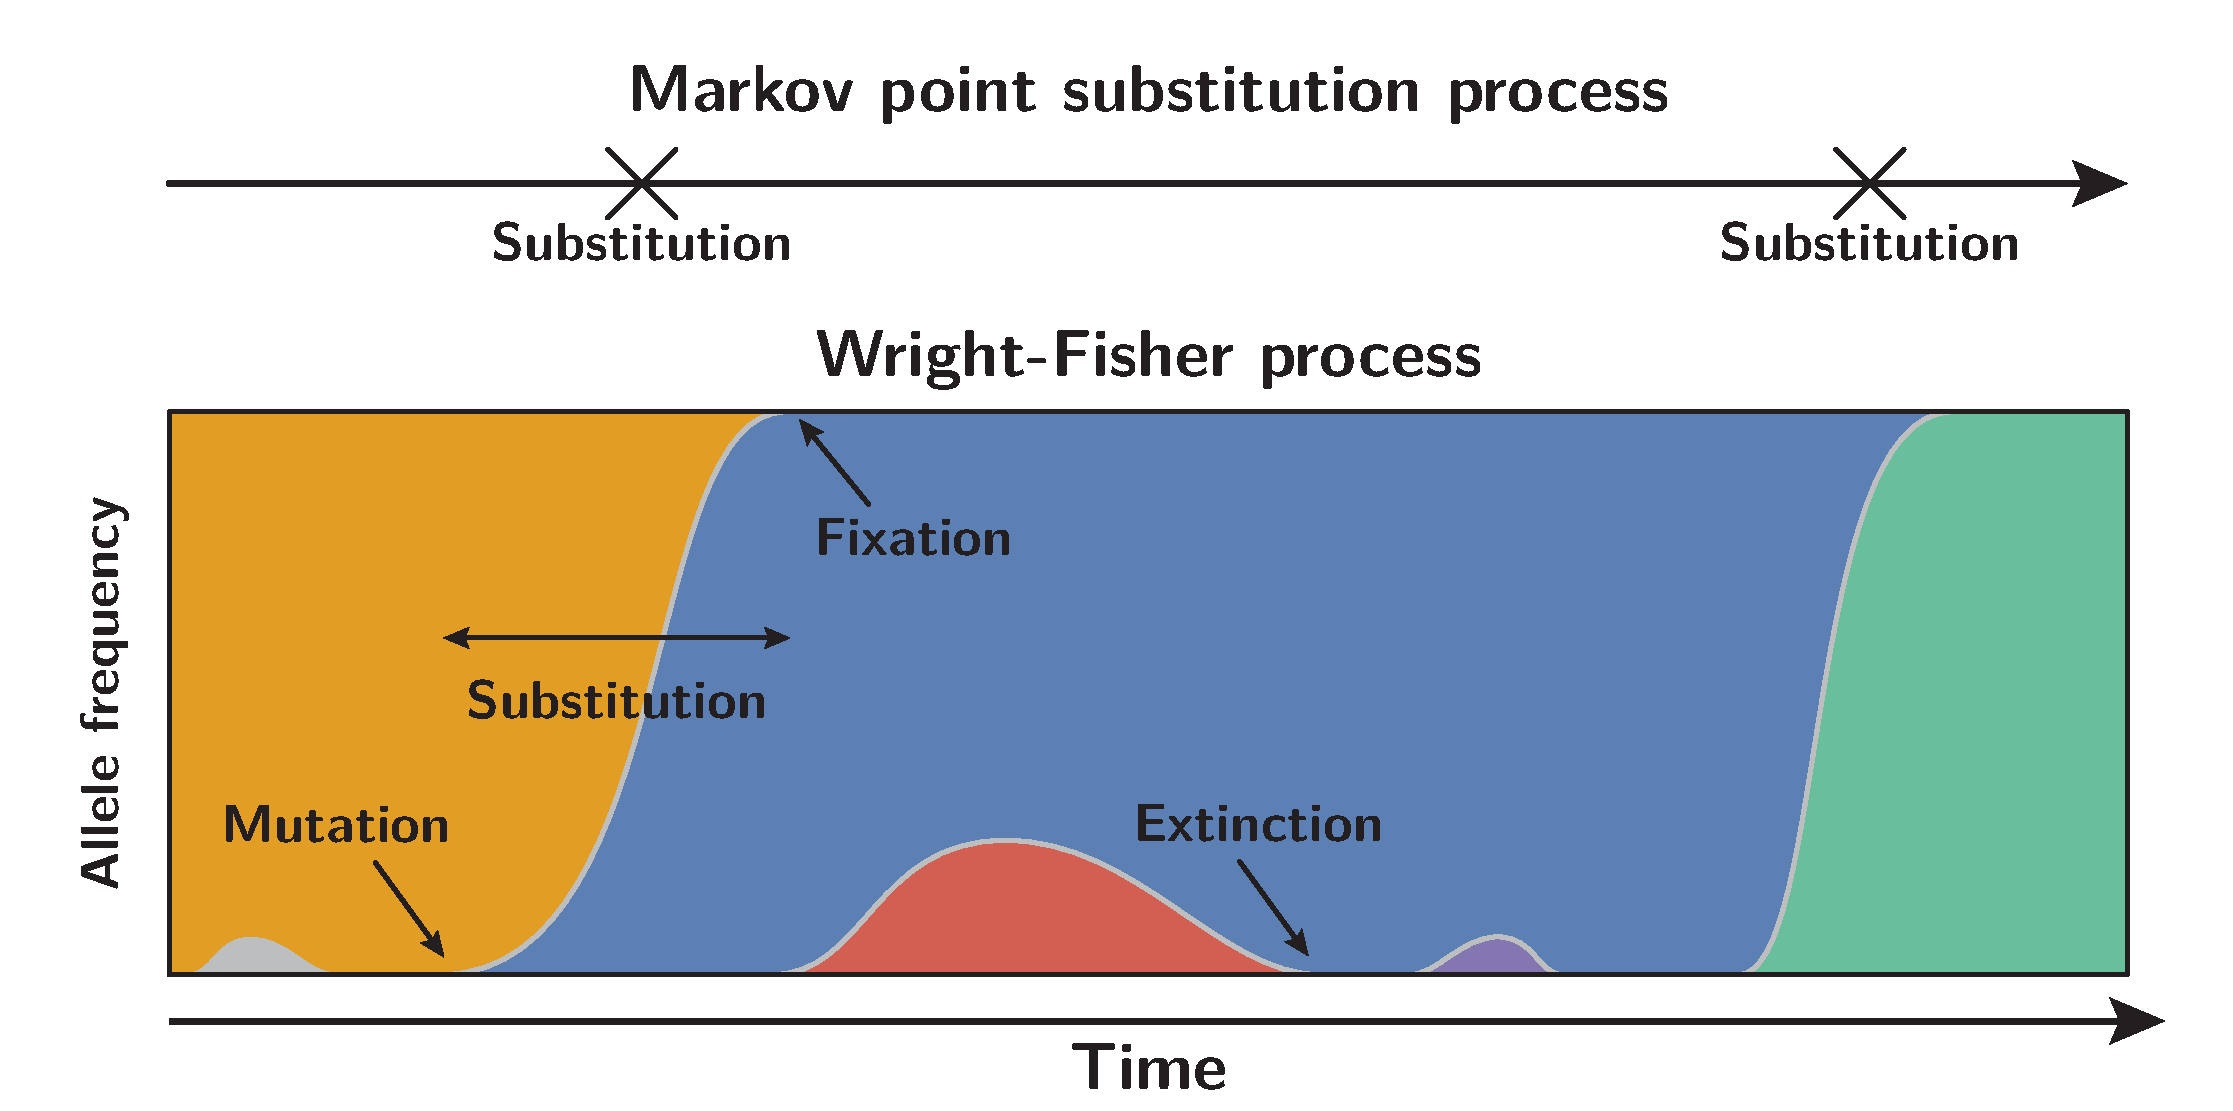
\includegraphics[width=0.6\textwidth]{figures/point-process.pdf}
	\caption[Mutation-selection point substitutions]{Mutation-selection point substitutions models. The trajectory of alleles inside a population is collapsed into a single point \gls{substitution} process. This approximation is valid under low mutation rate such that a mutation originate uniquely whenever the gene is monomorphic (with a single allele).}
\end{figure}

\subsection{Substitution rate}
The continuous-time Markov chain is defined by the instantaneous rate at which pair of states are transitioning.
Given the current state of the process is allele $A$, the rate of transition to other states can derived with population-genetics equations derived above.
At each generation, the expectation for the number of possible mutants is $2\Ne u$, and each of these mutant have a probability $P_{\mathrm{fix}}$ to result in a \gls{substitution}.
Altogether, the rate of \gls{substitution} from \gls{allele} $A$ to $B$, denoted $Q_{A \to B}$, is equal to the rate of mutation ($\mu_{A \to B}$) multiplied by the probability of fixation of the mutation $P_{\mathrm{fix}}(s_{A \to B}, \Ne)$ and scaled by the number of possible mutants at each generation ($2\Ne$):
\begin{align}
Q_{A \to B} & = 2 \Ne \mu_{A \to B}  P_{\mathrm{fix}}(s_{A \to B}, \Ne) \\
\end{align}
It is important to note that the \gls{substitution} rate and mutation rate are in the same unit, such that this equation is valid whether the rate is measured in unit of time or generation.
As a convention, mutation rate measured in unit of generation is denoted $u$, and denoted $\mu$ when measured in unit of time. As a consequence, $\submatrix$ is measured in unit of time in our equation.

In the case of \gls{neutral} mutations, the probability of fixation is independent of the original and target sequence, and equal $1/2 \Ne$. Finally the substitution rate $Q_{A \to B}$ simplifies to: 
\begin{align}
Q_{A \to B} & = 2 \Ne \mu_{A \to B}  P_{\mathrm{fix}}(0, \Ne) \\
Q_{A \to B} & = 2 \Ne \mu_{A \to B} \dfrac{1}{2\Ne} \\
Q_{A \to B} & =  \mu_{A \to B}
\end{align}
In the case of selected mutations, the probability of fixation depends on the difference of log-fitness ($f_i$ and $f_j$) between the two alleles:
\begin{align}
Q_{A \to B} & = 2 \Ne \mu_{A \to B} P_{\mathrm{fix}}(s_{A \to B}, \Ne) \\
			& = 2 \Ne \mu_{A \to B}  \dfrac{2(f_{B} - f_{A})}{1 - \e^{4\Ne(f_{A} - f_{B})} } \\
			& = \mu_{A \to B} \dfrac{F_{B} - F_{A}}{1 - \e^{F_{A} - F_{B}} }\text{, where } F = 4\Ne f \label{eq:sub-transion-rates}
\end{align}

It is important to note that if the difference of log-fitness tends to $0$, the \gls{substitution} rate equal the mutation rate:
\begin{align}
\lim_{|F_{B} - F_{A}| \to 0} Q_{A \to B} & = \mu_{A \to B}   \dfrac{F_{B} - F_{A}}{{1 - (1 + {F_{A} - F_{B}}) }} \nonumber \\
& =  \mu_{A \to B} 
\end{align}


Taken together, the transition rates which generates the \gls{substitution} history and ultimately the inter-specific diversity is parameterized solely by mutation, selection and drift.
Consequently, from a particular history of substitutions, one can theoretically estimate the parameter of selection, mutation and drift.

\subsection{Reversibility of the process}

The continuous-time Markov chain, defined by the transition rates between all possible alleles (equations \ref{eq:sub-transion-rates}) is irreducible, meaning it is always possible to go from any allele to any other possible allele, possibly in several substitutions.
Moreover, this substitution process is positive recurrent and aperiodic since any strictly positive transition rate is matched by a stricly positive transition for the reverse substitution.
More precisely, the substitution rate between two alleles is null only if the underlying mutation rate is null, in which case the transition rate for the reverse mutation is also null, hence the transition rate for the reverse substitution is also null.

Moreover, for an irreducible, positive recurrent and aperiodic continuous-time Markov chain, a necessary and sufficient condition to be reversible is given by Kolmogorov's criterion.
Kolmogorov's criterion implies that the product of transition rates through any closed loop is the same whenever the traversing is done forward or in reverse.
As an example for a Markov chain composed of $3$ alleles ($A$, $B$ and $C$) the transitions rate must satisfies the equality:
\begin{equation}
Q_{A \to B}Q_{B \to C}Q_{C \to A} = Q_{A \to C}Q_{C \to B}Q_{B \to A}
\end{equation}

\begin{figure}[htb!]
	\begin{center}
		\begin{tikzpicture}[->,>=stealth',auto,node distance=1.2cm and 1.6cm,semithick]
		\tikzstyle{every state}=[]
		
		\node[] (0) {};
		\node[state] (A) [above=of 0] {$A$};
		\node[state] (B) [below left=of 0] {$B$};
		\node[state] (C) [below right=of 0] {$C$};
		
		\path[->]
		(A) edge [BLUE,bend right=45] node [left] {$Q_{A \to B}$} (B)
		(B) edge [BLUE,bend right=45] node [below] {$Q_{B \to C}$} (C)
		(C) edge [BLUE,bend right=45] node [right] {$Q_{C \to A}$} (A)
		(B) edge [RED,bend right=15] node [left] {$Q_{B \to A}$} (A)
		(C) edge [RED,bend right=15] node [below] {$Q_{C \to B}$} (B)
		(A) edge [RED,bend right=15] node [right] {$Q_{A \to C}$} (C);
		\end{tikzpicture}
	\end{center}
	\caption[Kolmogorov's criterion]{The continuous-time Markov chain is reversible if the process fulfills Kolmogorov's criterion, such that the product of transition rate for a closed loop is equal whether traversed in one sens (blue arrows) or the other (red arrows).}
	\label{fig:reversible-circuit}%
\end{figure}

From transition rates of the substitution process (\ref{eq:sub-transion-rates}), Kolmogorov's criterion can be derived as:
\begin{align}
\dfrac{Q_{A \to B}Q_{B \to C}Q_{C \to A}}{Q_{A \to C}Q_{C \to B}Q_{B \to A}}
={}& \dfrac{\mu_{A \to B}\mu_{B \to C}\mu_{C \to A}}{\mu_{A \to C}\mu_{C \to B}\mu_{B \to A}}
	 \times \dfrac{(F_{B} - F_{A})(F_{C} - F_{B})(F_{A} - F_{C})}{(F_{C} - F_{A})(F_{B} - F_{C})(F_{A} - F_{B})} \notag \\
	 &\ \times \dfrac{( 1 - \e^{F_{A} - F_{C}} )( 1 - \e^{F_{C} - F_{B}} )( 1 - \e^{F_{B} - F_{A}} )}{( 1 - \e^{F_{A} - F_{B}} )( 1 - \e^{F_{B} - F_{C}} )( 1 - \e^{F_{C} - F_{A}} )}, \\
={}& - \dfrac{\mu_{A \to B}\mu_{B \to C}\mu_{C \to A}}{\mu_{A \to C}\mu_{C \to B}\mu_{B \to A}} \notag \\
&\ \times \dfrac{\e^{F_{A}}( \e^{-F_{A}} - \e^{ - F_{C}} )\e^{F_{C}}( \e^{-F_{C}} - \e^{ - F_{B}} )\e^{F_{B}}( \e^{-F_{B}} - \e^{ - F_{A}} )}{\e^{F_{A}}( \e^{-F_{A}} - \e^{ - F_{B}} )\e^{F_{B}}( \e^{-F_{B}} - \e^{ - F_{C}} )\e^{F_{C}}( \e^{-F_{C}} - \e^{ - F_{A}} )}, \\
={}& \dfrac{\mu_{A \to B}\mu_{B \to C}\mu_{C \to A}}{\mu_{A \to C}\mu_{C \to B}\mu_{B \to A}}.
\end{align}
As a result, Kolmogorov's criterion for the substitution process is satisfied only if the mutation process is also reversible, in which case Kolmogorov's criterion is also fulfilled:
\begin{equation}
\mu_{A \to B}\mu_{B \to C}\mu_{C \to A}=\mu_{A \to C}\mu_{C \to B}\mu_{B \to A}.
\end{equation}
This example can be generalized for any close loop, such that the reversibility of the substitution process is conditioned on the reversibility of the underlying mutation process, which is often assumed.

\subsection{Stationary distribution}

A realization of the \gls{mc} for a long period of time results in a given proportion of the time for which the process is fixed for a specific allele, where this proportion depends of the allele fitnesses, the mutational process and $\Ne$.
Because the continuous-time \gls{mc} is irreducible, positive recurrent and aperiodic, it has a unique stationary distribution $\bm{\pi}$ where $\pi_{A}$ corresponds to the proportion of time spent in allele $A$ after the Markov chain has run for an infinite amount of time. 

Moreover, under the condition that the \gls{mc} is time-reversible, the detailed balanced for the stationary distribution is satisfied:
\begin{align}
\dfrac{\pi_{A}}{\pi_{B}} & = \dfrac{Q_{B \to A}}{Q_{A \to B}} \\
& = \dfrac{\mu_{B \to A}}{\mu_{A \to B}}  \dfrac{F_{A}-F_{B}}{ 1 - \e^{F_{B}-F_{B}}}  \dfrac{1 - \e^{F_{A} - F_{B}} }{F_{B} - F_{A}}\\
& = - \dfrac{\mu_{B \to A}}{\mu_{A \to B}}  \dfrac{ \e^{F_{A}}(\e^{-F_{A}} - \e^{- F_{B}}) }{ \e^{F_{B}}(\e^{-F_{B}} - \e^{- F_{A}})}  \\
& = \dfrac{\mu_{B \to A}}{\mu_{A \to B}} \dfrac{\e^{F_{A}}}{\e^{F_{B}}} \\
\end{align}
Under the assumption that the mutational process is also reversible, the detailed balanced for the stationary distribution of the mutation process ($\backref{\sigma}$) is satisfied:
\begin{align}
\dfrac{\mu_{B \to A}}{\mu_{A \to B}} & = \dfrac{\sigma_{A}}{\sigma_{B}} 
\end{align}
Altogether, the probability $\pi_{A}$ to find the population in allele $A$ is proportional to a function (also called a Boltzmann factor) that depends only on the fitness of allele $A$, the population size, and details of the mutation process \citep{Sella2005,Mustonen2005}:
\begin{align}
\dfrac{\pi_{A}}{\pi_{B}} & = \dfrac{\sigma_{A}\e^{F_{A}}}{\sigma_{B}\e^{F_{B}}} \text{ and } \sum_{A}\pi_{A} = 1, \\ 
\iff \pi_{A} & = \dfrac{\sigma_{A}\e^{F_{A}}}{\sum_{B} \sigma_{B}\e^{F_{B}} }, \label{eq:equilibrium-mut-sel}
\end{align}
where the denominator is a normalizing constant such that the sum of probabilities equal to $1$.
In analogy to thermodynamic systems, the evolutionary system reaches thus a Boltzmann-like distribution with $\Ne^{-1}$ playing the role of evolutionary temperature, and the log-fitness $f$ the role of energy\footnote{At high mutation rates, the quasi-species theory provides another analogy with statistical mechanics, in which the mutation rate plays the role of temperature instead of genetic drift.}.

\subsection{Equilibrium substitution rate over mutation rate} 

Probabilities of the stationary distribution allows to calculate all observable quantities of interest, such as mean fitness, mean mutation and \gls{substitution} rates, using standard probability theory.
One quantity of interest is the \gls{substitution} rate of selected mutations relative to that of \gls{neutral} mutations, called $\langle \nu \rangle$.
From its definition, $\langle \nu \rangle=1$ for genes or sites under \gls{neutral} evolution.
Most importantly, departure from $1$ would be interpreted as a signature of selection on sequences. 
First, $\langle \nu \rangle>1$ is interpreted as a signal of adaptive recurrent evolution, where selection coefficient are on average positive.
On the other hand, $\langle \nu \rangle<1$ is a signal of underlying purifying selection, such that the sequence is constrained and mutations proposed have on average a negatively selection coefficient.
Together, in the case of a mutation-selection point \gls{substitution} process, $\langle \nu \rangle$ is defined as:
\begin{equation}
\label{eq:relative-sub-rate}
\langle \nu \rangle = \dfrac{ \sum_{A} \pi_{A} \sum_{B} Q_{A \to B}}{\sum_{A} \pi_{A}  \sum_{B} \mu_{A \to B}},
\end{equation}
where the notation $\langle . \rangle$ denotes the statistical average.
It worth noting that under the assumption of a static fitness landscape, a mutation-selection point \gls{substitution} process will result in $\langle \nu \rangle \leq 1$ \citep{Mustonen2009}. 

\begin{table}[H]
	\resizebox{\columnwidth}{!}{%
		\begin{tabular}{|l|c|c|c|}
			\hline
			\textbf{Parameter} & \textbf{Symbol} & \textbf{Range} \\
			\hline\hline
			Scaled fitness & $F=4 \Ne f$ & finite, positive or negative \\
			\hline Mutation rate per time & $\mu$ & $[10^{-11}, 10^{-8}]$ per site per year \\
			\hline Substitution rate per time & $Q$ & $[10^{-11}, 10^{-8}]$ per site per year \\
			\hline Equilibrium frequency & $\pi$ & $[0, 1]$ \\
			\hline Equilibrium frequency under mutation & $\sigma$ & $[0, 1]$ \\
			\hline Equilibrium substitution rate & \multirow{2}{*}{ $\langle \nu \rangle$} & \multirow{2}{*}{$[0, 1]$ for purifying selection} \\
			over mutation rate & & \\
			\hline
		\end{tabular}}
	\caption[Parameter of mutation-selection processes]{Parameter of mutation-selection processes}\label{table:params-mutsel}
\end{table}

\section{Mutation-selection analogy}

This section develops reflections on apparent similarities and analogies between the mutation-selection process and other processes present in a variety of scientific fields outside of evolutionary biology, displaying the same underlying mechanism and emerging properties, though with different name and aspiration.
This effort is made in the aim of giving another view of the mutation-selection process, such as to better appreciate and conceptualize its assumptions, its limits, and the respective role of the different components. 
Such attempts requires to boil down the mutation-selection mechanism into its core components, while at the same time rephrasing the description using lexicography outside of population-genetic such as to open new perceiving angles.

At the bottom, mutation is a process creating diversity, changing and moving the current viable state to a novel and unknown position, fundamentally allowing exploration of the state space.
On the other hand, selection is the criteria on which a new state is deemed a disrupting innovation or a nonviable alteration, and allow to determine which changes to exploit and which to filter out and discard based on its fitness.
Fundamentally, reducing the diversity created by the mutation process is the very essence of selection.
Finally, drift arbitrate between the creation and reduction of the two processes, it dictates how much exploration of novelty is permitted, and conversely how much exploitation of only the fittest states is granted.

I argue that this creation and reduction process is found at the core of several research disciplines, while the link between them is scarcely made \citep{Baeck1994, Eiben1998}. 

\subsection{Metropolis-Hasting sampling}
Obtaining a sequence of random samples from a probability distribution can be difficult, especially when the number of dimensions is high.
However, the Metropolis-Hasting procedure based on a Monte Carlo \gls{mc} can sample from any probability distribution, provided that we know how to compute the probability density, or even less restrictively any function proportional to the density \citep{Hastings1970}.
This stochastic procedure which is based on three steps bears many similarities with the mutation-selection process:
\begin{itemize}
	\item Generate a stochastic candidate from the current state, analogous to the mutation.
	\item Calculate the acceptance ratio as the ratio of the two densities, analogous to the selection coefficient of the mutated state.
	\item Stochastic acceptance or rejection based on the acceptance ratio, a process analogous to drift. 
\end{itemize}
Inherently, Metropolis-Hasting procedure is based on creating and subsequently reducing diversity, which allows to obtain a random sequence of samples from any distribution with a straightforward recipe, and is a critical tools in statistic and statistical physics.

\subsection{The exploration-exploitation dilemma}
Many mathematical, engineering and day-life problems are not about sampling a state space, but rather finding the optimal and best state given a criteria or a function to maximize.
Naturally, we would prefer deterministic (strictly reproducible) rather than stochastic optimizing strategies to search for an optimal state.
Unfortunately, whenever the state space is too large, often due to the curse of dimensionality, a greedy or heuristic search of an optimal state can performs atrociously \citep{Bellman1966}.
In high dimensional space, stochastic optimization tools have been deemed very valuable, such as stochastic gradient decent or so called evolutionary algorithm \citep{Russell2010,Vikhar2017}.
Inherently, they are based on two processes, one is stochastically creating diversity and exploring the state space, while the other is filtering the explored states and thus reducing the diversity.

In the constrained case of a finite number of time or attempts to find the best outcome overall, the problem is best described by the multi-armed bandit problem. The name comes from imagining a gambler at a row of slot machines (sometimes known as one-armed bandits), where each slot machine provides a random reward from a probability distribution specific to that machine. The player has to decide which machines to play, how many times to play each machine and in which order to play them, and whether to continue with the current machine or try a different machine, such as to maximize the sum of rewards earned through a sequence of trials.
The gambler faces a dilemma at each trial, either reducing his regret by exploiting the best arm, or gaining information through exploration of other arms.
The best strategy to solved this dilemma can be mathematically derived in numerous cases, and encompass a mixing strategies with a defined ratio of exploration and exploitation \citep{Auer2002,Kocsis2006,Furnkranz2006}.
This problem is far from be only theoretical, and has be used to explain a multitude of phenomena, such as the movement of animals in novel landscapes, the most efficient resource allocation for a start-up company, the effects of age on knowledge acquisition in humans, and in search of the most efficient treatment in clinical trials (hence the name a clinical arm) \citep{Berger-Tal2014, March}. 
An other application of the exploration-exploitation dilemma is AlphaGo, the first computational program mastering the board game go at the professional 9-dan level in 2017, and out-compete Ke Jie, the world n°1 ranked player at the time \citep{Silver2017, Silver2018}.
AlphaGo has often been publicized and hyped in various media outlets that this feat was possible due to machine learning, more specifically due to convolutionnal neural networks.
However, it is more scarcely mentioned that AlphaGo neural network is combined with an exploration-exploitation algorithm, or more specifically Monte Carlo tree search. 
In practice, the convolutionnal neural network is used as a criteria to measure the advantage of a board configuration\footnote{Convolutionnal neural networks also use a stochastic gradient descend to reach convergence, inherently leveraging stochastic exploration and exploitation procedure to optimize the parameters of the neural network.}, but the different moves and path probed and trimmed is done via an exploration-exploitation procedure. 


Altogether, exploration and exploitation, creation and reduction, mutation and selection, are different names that encompass the inherently same process efficiently sampling and optimizing whenever the state is too large to be traversed.
I argue that scientific research endeavor is also a exploration-exploitation dilemma, which is arguably externally pressured to pursue exploitation, through funding of impactful research and a \textit{publish-or-perish} systemic culture in early career stage.

% As a side note, it appears that drift and selection are actually confounded, they are both on the side of exploitation, not on exploration.
As a side note, mutation is a necessary process of evolution, while sexe is not mandatory but increase the diversity of genomes between generations.
Arguably, studying evolution while disregarding mutation is a sufficient approximation whenever mutation rate and number of generations is low, which is developed thoroughly through the whole field of quantitative genetics.
Sex and mutation are both generating new states and are part of the more general exploration facet.
This explains why sex is favored in fluctuating environments.

I argue that evolutionary biologists, studying and leveraging the pervasive process of mutation and selection, can gain knowledge by recruiting insight and developments from other fields, much like there as been many crossover between economics and evolution in the context of game theory.\footnote{Game theory had originally been developed to model economic actors behavior and strategies \citep{VonNeumann1947}, while latter being emerging as the framework of evolutionary dynamics, which explains the emergence of altruistic behaviours in Darwinian evolution \citep{Smith1973, Smith1982, Nowak2006}.}.

As an example of such insight from exploration-exploitation dilemma is on the understanding of relationship between mutation rate and chromosome size.
It has been observed that organism with a low mutation rate (per site per generation) tend also to have a long chromosome size, such that the product of genome size and mutation rate is constant \cite{Drake1991}.
An explanation for this pervasive negative correlation between mutation rate and genome size invoke the drift barrier hypothesis, where the correlation is inherently due to an underlying changes of genetic drift \citep{Lynch2016a}.
The drift barrier hypothesis posits the selection operates to minimize the mutation rate, with the efficiency of such improvement eventually being overcome by random genetic drift, such that population with higher population size have smaller mutation rate. 
On the other hand, higher population size induces stronger purifying selection which reduce genome size by expelling transposable elements.
Altogether, both high mutation rate and smaller genome are consequences of higher population size.
An alternative explanation for the negative correlation between mutation rate and genome size is that for each new generation, the genetic diversity of offsprings must balance the trade-off between exploration of new genotype and the reliable transmission of the current one.
The genetic difference between parents and offsprings is the product of mutation rate and genome size, such that individuals whom are not robust enough undergo deleterious mutations and disappear, whereas individuals whose genotypes are not variable enough are outcompeted by those that were able to discover innovations \citep{Knibbe2007, Beslon2010, Hindre2012, Batut2014, Biller2016}.


